\section{Approach}
\label{cha:approach}

The following chapter presents the methodological approach of this thesis. While the subsequent chapter discusses the concrete implementation aspects, this section establishes the theoretical foundation that builds upon the concepts introduced in chapter \ref{cha:background}. The structure of this chapter follows the sequence of steps illustrated in Figure \ref{fig:04-overview}, beginning with an outline of the central objective of the thesis. This is followed by a set of assumptions that define the scope, applicability, and limitations of the proposed approach. The remainder of the chapter then describes each step in detail, explaining how the individual components contribute to the overall objective of enabling energy-aware and contention-conscious co-location of scientific workflow tasks.

\subsection{Central Objective}
\label{sec:central_objective}

The central objective of this work is to model the co-location of scientific workflow tasks with a focus on achieving energy-awareness and determining how this knowledge can be applied during workflow execution to improve resource utilization and overall energy efficiency. To accomplish this, we introduce two key concepts: (i) \textit{ShaReComp} and (ii) \textit{ShaRiff}. Both address the idea of shared resource usage but from different perspectives. \textit{ShaReComp} defines the modeling approach for resource sharing during computation. It focuses on understanding and representing co-location with respect to resource usage, contention, and energy behavior. In contrast, \textit{ShaRiff} introduces an algorithmic framework that applies the \textit{ShaReComp} model during workflow execution to enable informed and feasible resource sharing. Together, these concepts provide both the theoretical foundation and practical mechanism for energy-aware co-location in scientific workflows.
\textit{ShaReComp} is inspired by the work presented in \cite{5644899}, which introduced a mathematical formulation of the co-location problem. However, the implementation of \textit{ShaReComp} differs significantly in its scope and application. By combining \textit{ShaReComp} with \textit{ShaRiff}, this work aims to investigate how co-location can be directly integrated into the dynamic scheduling and task mapping process, emphasizing that co-location and scheduling are inherently interdependent and should be addressed jointly. To achieve this, workflow tasks are characterized prior to execution, enabling contention-aware co-location decisions at runtime. In this setting, co-location is implemented at the virtual container level, focusing on virtual machines deployed on physical hosts. Additionally, this work extends the scope of co-location from merely determining which tasks should share resources to understanding how the performance behavior of co-located tasks can be modeled and predicted, thereby providing actionable insights for resource managers in future workflow executions.

% Figure Approach Overview
\begin{figure}[H]
    \centering
    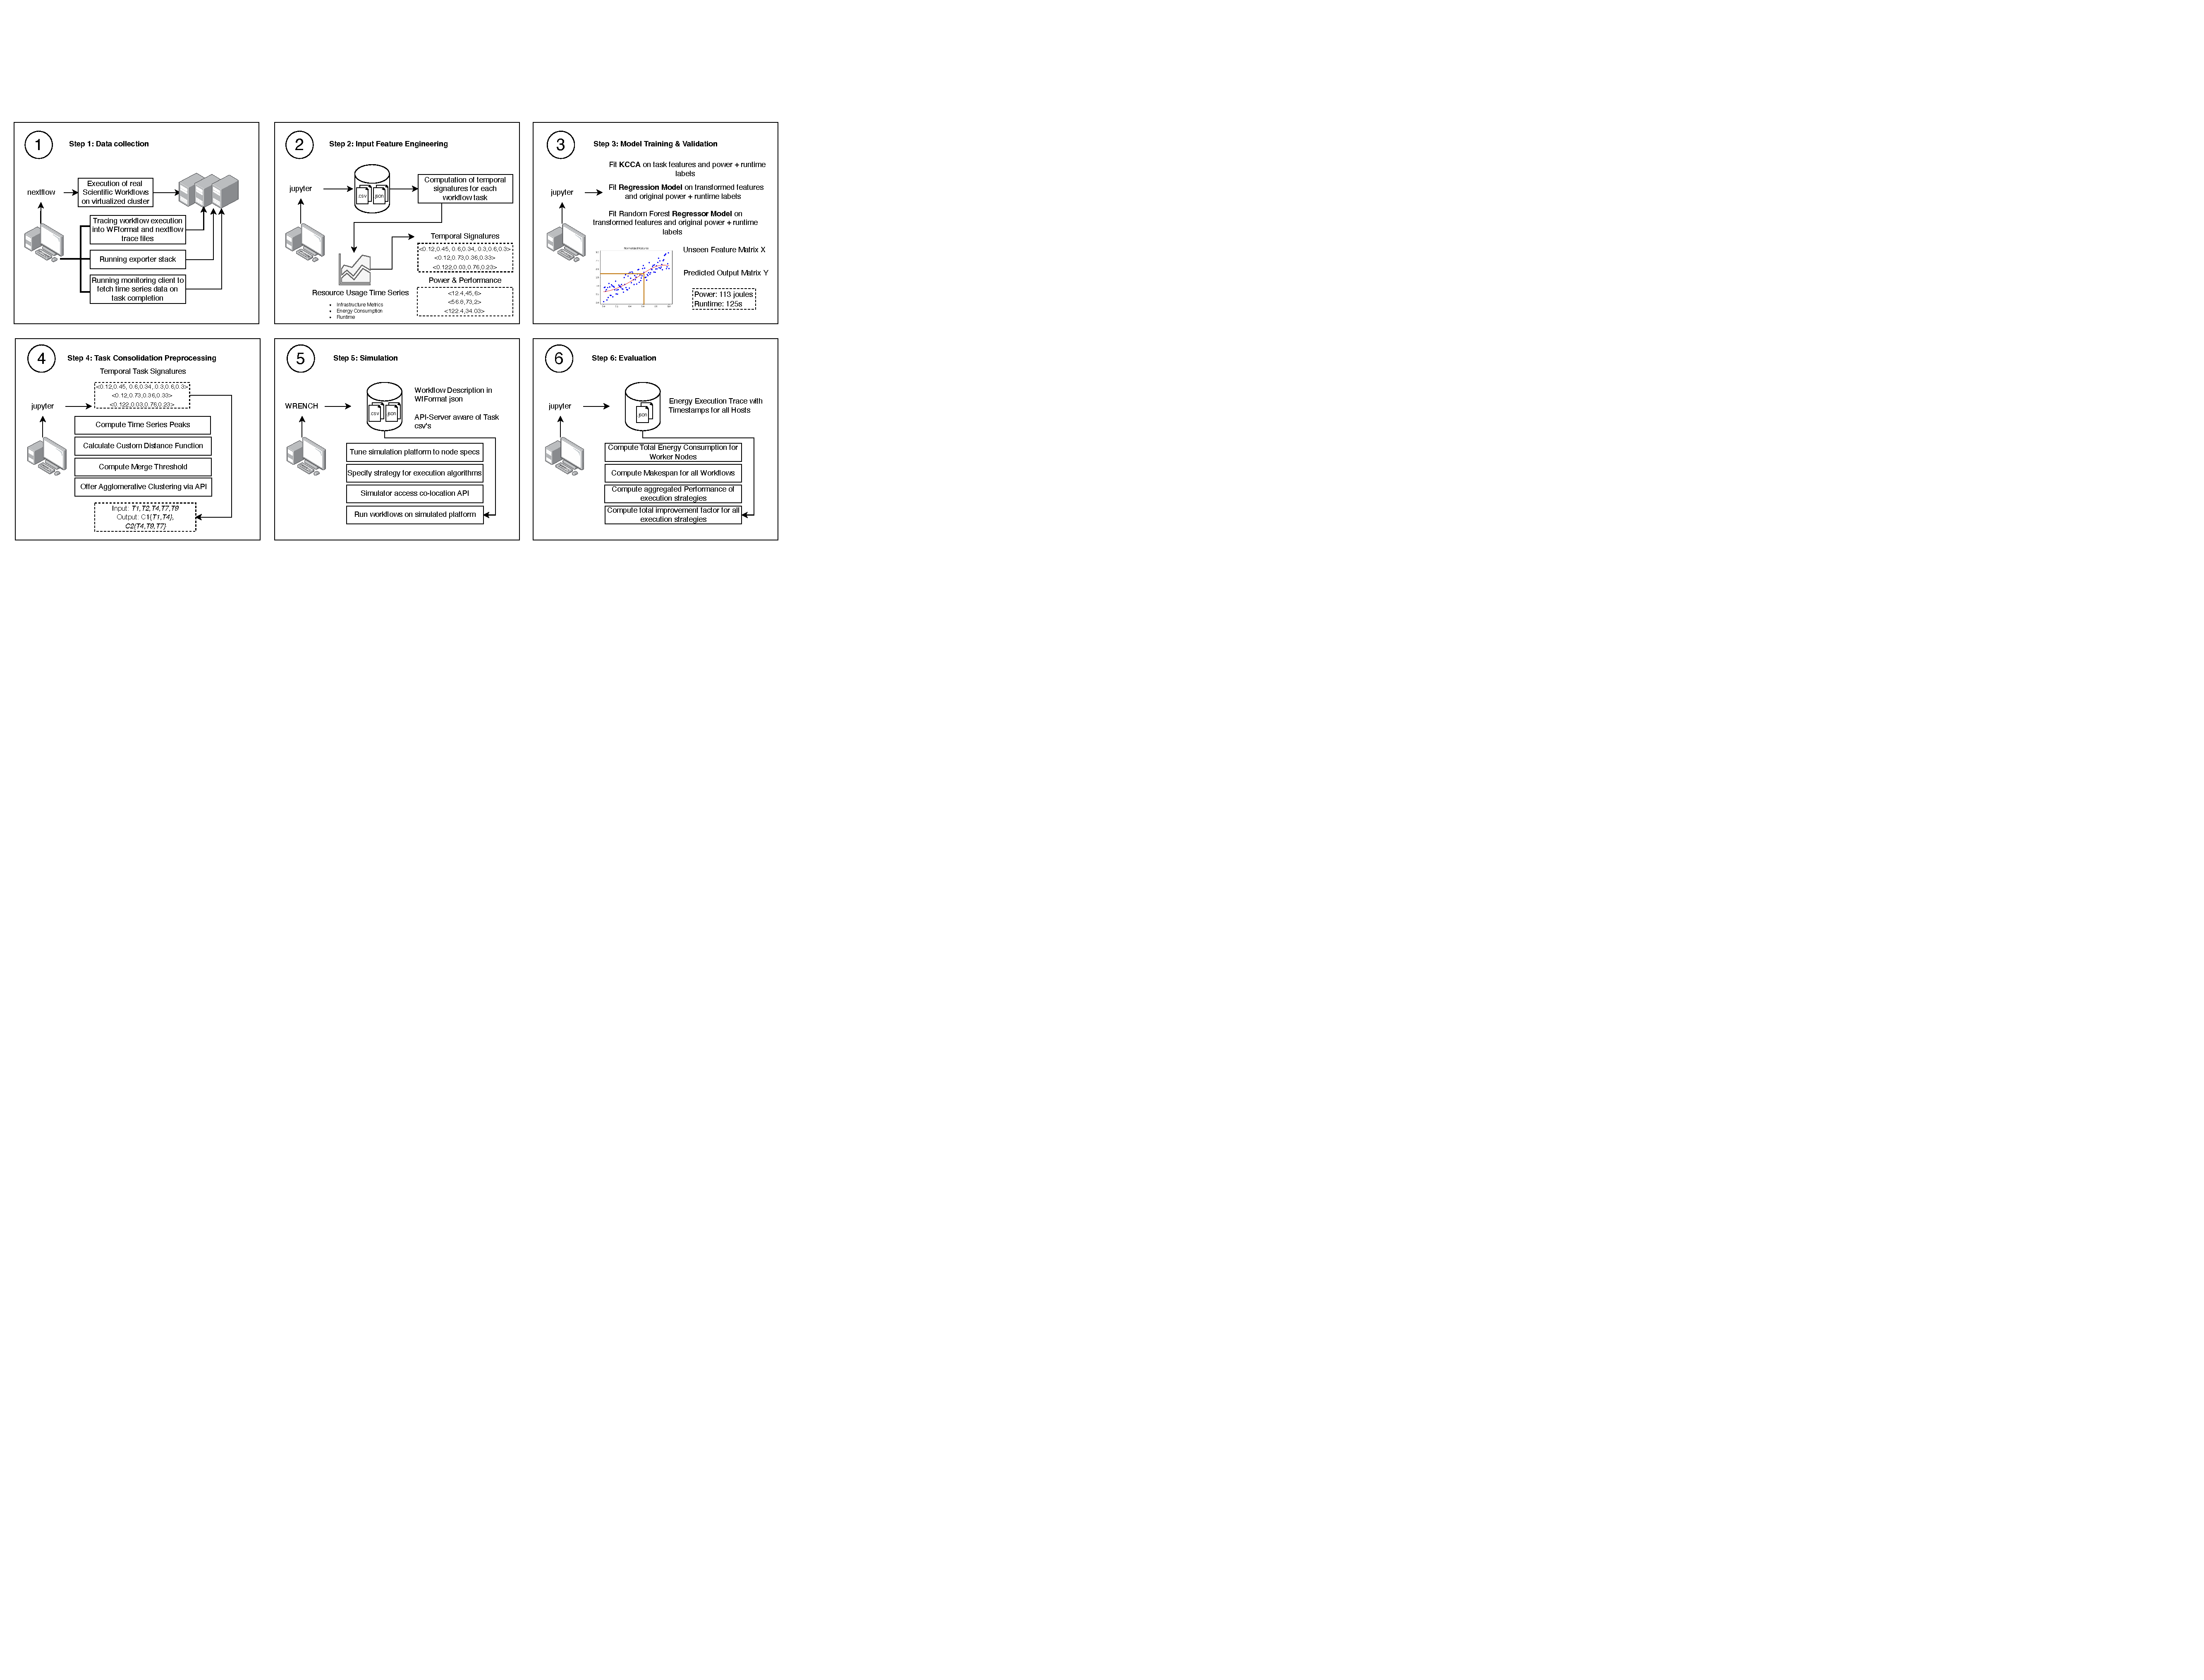
\includegraphics[scale=0.45]{fig/04/04-overview.pdf}
    \small
    \caption{Overview of the Proposed Approach}
    \label{fig:04-overview}
    \tiny
    The proposed approach consists of 6 steps.
\end{figure}

The proposed objective, introduced in Section \ref{subse:problem_motivation_description}, is decomposed into six main steps, as illustrated in Figure \ref{fig:04-overview}. Step 1, described in Section \ref{sec:online_task_monitoring}, involves a data collection phase that captures detailed execution metrics from scientific workflow runs. In Step 2, this collected data undergoes structural processing and formatting to extract relevant performance characteristics, as outlined in Section \ref{sec:data_preprocessing_general}. The raw data treatment of Step 2 is performed immediately after data collection, while Steps 3 and 4 require more specialized data preparation tailored to their respective analytical goals. Details for these stages are provided in Sections \ref{sec:data_preprocessing_clustering} and \ref{sec:data_preprocessing_predictive}.
Step 3 focuses on consolidating time-series data by identifying tasks with complementary resource usage patterns through clustering, as discussed in Section \ref{sec:task_clustering}. Step 4 reorganizes the data collected in Step 1 into a format suitable for learning the relationship between task behavior, runtime, and energy consumption, as described in Section \ref{sec:prediciton_kcca_rfr}. Finally, Steps 5 and 6, presented in Section \ref{sec:simulation_environment}, demonstrate how the theoretical concepts developed in Step 3 can be applied during workflow execution and how their potential benefits in terms of performance and energy efficiency can be evaluated through simulation.

% Assumptions or Disclaimers
\subsubsection{Assumptions}
\label{sec:assumptions}

To outline the scope, boundaries, and methodological constraints of this work, the following guiding assumptions were defined:

\begin{enumerate}
    \item \textbf{Monitoring Configuration Limits}: Workflow tasks are described by 80 monitoring features. This work does not investigate the influence of monitoring data dimensionality on clustering and predictive performance.
    \item \textbf{Monitoring Data Coverage}: Short-lived tasks under one second are only partially captured or occasionally missed due to high system load and sampling intervals exceeding one second during workflow execution.
    \item \textbf{Offline Data Analysis}: The data preprocessing and predictive model fitting are performed offline after workflow execution. The co-location clustering algorithm is evaluated offline but also transformed into a suitable format for integration into the simulation environment.
    \item \textbf{Simulation Environment and Platform Equivalence}: The simulated platform is assumed to approximate the physical execution environment. It is expected that the overall behavior observed in simulation aligns with real-world execution trends.
    \item \textbf{Simulation Capabilities and Contention Modelling}: The WRENCH framework currently supports simulation of memory contention by limiting per-Host memory consumption, where exceeding the limit results in extended task execution times. Similarly, CPU contention is modeled through proportional increases in task runtime. Other low-level contention effects like cache interference, interconnect bottlenecks, or I/O contention are not modeled in this iteration. The energy model provided by SimGrid is assumed to realistically approximate energy consumption variations when tasks with differing resource usage profiles are co-located on the same virtual machine. The impact on energy efficiency is attributed to CPU utilization behavior and derived from the platform description where different load levels map to consumed energy amount.
\end{enumerate}

\subsection{Online Task Monitoring}
\label{sec:online_task_monitoring}

The online task monitoring approach builds on a hierarchical architecture designed to capture a broad range of metrics relevant to the execution of scientific workflows. Its design is inspired by \cite{Bader_2022} and follows a four-layered structure comprising the Resource Manager, Workflow, Machine, and Task layers. Each layer represents a distinct level of abstraction within the workflow execution environment, providing insights into specific aspects of system performance and resource utilization.

Table \ref{tab:monitoring_sources_updated} provides an overview of the tools and data collection options that we considered for achieving our monitoring objectives, outlining how different metrics could be gathered and integrated across the hierarchical layers to form a comprehensive view of workflow behavior.

\begin{table}[H]
    \centering
    \renewcommand{\arraystretch}{1.15}
    \resizebox{\textwidth}{!}{
        \begin{tabular}{
            p{4cm}
            >{\centering\arraybackslash}p{1.8cm}
            >{\centering\arraybackslash}p{1.8cm}
            >{\centering\arraybackslash}p{1.8cm}
            >{\centering\arraybackslash}p{1.8cm}
            >{\centering\arraybackslash}p{1.8cm}
            >{\centering\arraybackslash}p{1.8cm}
            >{\centering\arraybackslash}p{1.8cm}
            }
            \toprule
            \textbf{Metric Category}         & \textbf{cAdvisor} & \textbf{Deep-Mon} & \textbf{docker-activity} & \textbf{scaphandre} & \textbf{slurm-exporter} & \textbf{process-exporter} & \textbf{cgroups-exporter} \\
            \midrule

            \multicolumn{8}{l}{\textbf{Workflow-Level Metrics}}                                                                                                                                                         \\[3pt]
            Infrastructure status            &                   &                   &                          &                     & x                       &                           &                           \\
            Running workflows                &                   &                   &                          &                     & x                       &                           &                           \\
            Workflow ID                      &                   &                   &                          &                     & x                       &                           &                           \\
            File system status               &                   &                   &                          &                     & x                       &                           &                           \\

            \midrule
            \multicolumn{8}{l}{\textbf{Machine-Level Metrics}}                                                                                                                                                          \\[3pt]
            Status                           &                   &                   &                          & x                   & x                       &                           &                           \\
            Machine type                     &                   &                   &                          & x                   & x                       &                           &                           \\
            Hardware specification           &                   &                   &                          & x                   & x                       &                           &                           \\
            Available resources              &                   &                   &                          & x                   & x                       &                           &                           \\
            Used resources                   &                   &                   &                          & x                   & x                       &                           &                           \\
            Requested and consumed resources &                   &                   &                          & x                   & x                       &                           & x                         \\
            Resource usage metrics           &                   &                   &                          & x                   & x                       &                           & x                         \\
            Power consumption                &                   &                   &                          & x                   & x                       &                           &                           \\
            Fault diagnosis                  &                   &                   &                          &                     & x                       &                           &                           \\

            \midrule
            \multicolumn{8}{l}{\textbf{Task-Level Metrics}}                                                                                                                                                             \\[3pt]
            Task status                      & x                 & x                 &                          & x                   & x                       &                           &                           \\
            Task ID                          &                   &                   &                          &                     & x                       &                           & x                         \\
            Task duration                    & x                 & x                 &                          & x                   & x                       &                           &                           \\
            Requested and consumed resources & x                 & x                 & x                        & x                   & x                       &                           & x                         \\
            Resource usage metrics           & x                 & x                 & x                        & x                   & x                       &                           & x                         \\
            Process metrics                  &                   & x                 &                          & x                   &                         & x                         &                           \\
            Power consumption                &                   & x                 & x                        & x                   & x                       &                           &                           \\

            \bottomrule
        \end{tabular}
    }
    \small
    \caption{Overview of monitored metrics and their data sources inspired by \cite{Bader_2022}.}
    \label{tab:monitoring_sources_updated}
\end{table}
To enable access to detailed performance metrics in time-series format, Prometheus was selected as the central time-series database. As shown in Table \ref{tab:monitoring_sources_updated}, the monitoring setup therefore focused on tools that are interoperable with Prometheus as data exporters and that operate effectively within the layered monitoring framework.
During the evaluation of several potential exporters, some were excluded due to limited compatibility, excessive overhead, or incomplete metric coverage—particularly for short-lived or multi-process workflow tasks. After comparative testing, the combination of cAdvisor and a custom fork of the Deep-Mon system \cite{8425477} produced the most stable and comprehensive results across varying workloads and resource types. These two tools were therefore selected as the foundation of the final monitoring setup.

The following table presents the final selection of data sources that were retained for the monitoring setup, along with the specific metrics enabled for each source.

% Table with Tool Overview and metrics
\begin{table}[H]
    \centering
    \renewcommand{\arraystretch}{1.2}
    \setlength{\tabcolsep}{8pt}
    \small
    \begin{tabularx}{\textwidth}{
            >{\raggedright\arraybackslash}X
            >{\raggedright\arraybackslash}X
        }
        \toprule
        \textbf{Software Tool} & \textbf{Used Metrics} \\
        \midrule

        nextflow               &
        trace file summary                             \\

        \midrule
        cAdvisor               &
        container\_memory\_working\_set\_bytes,
        container\_memory\_usage\_bytes,
        container\_memory\_rss,
        container\_fs\_reads\_bytes\_total,
        container\_fs\_writes\_bytes\_total,
        container\_fs\_io\_current                     \\

        \midrule
        Deep-Mon               &
        container\_memory\_working\_set\_bytes,
        container\_memory\_usage\_bytes,
        container\_memory\_rss,
        container\_fs\_reads\_bytes\_total,
        container\_fs\_writes\_bytes\_total,
        container\_fs\_io\_current,
        container\_mem\_rss,
        container\_mem\_pss,
        container\_mem\_uss,
        container\_kb\_r,
        container\_kb\_w,
        container\_num\_reads,
        container\_disk\_avg\_lat,
        container\_num\_writes,
        container\_cycles,
        container\_cpu\_usage,
        container\_cache\_misses,
        container\_cache\_refs,
        container\_weighted\_cycles,
        container\_power,
        container\_instruction\_retired                \\

        \bottomrule
    \end{tabularx}%
    \small
    \caption{Metrics included in the workflow monitoring approach}
    \label{tab:monitoring-metrics}
\end{table}

% Description of cadvisor, ebpf-energy-monitor
cAdvisor is an open-source daemon for monitoring resource usage and performance of containers. It continuously discovers containers via Linux cgroups under the path /sys/fs/cgroup. Once started, cAdvisor subscribes to create/delete events in the cgroup filesystem, converts them to internal add/remove events, and configures per-container handlers. Metrics originate from machine-level facts parsed from /proc and /sys directories and most prominently container and process usage collected at cgroup boundaries. In practice, cAdvisor provides low-overhead, per-container telemetry \cite{cadvisor_github_2025}.

Deep-Mon is a per-thread power attribution method to translate coarse-grained hardware power measurements into fine-grained, thread-level energy estimates by exploiting hardware performance counters. The Intel RAPL interface provides power readings per processor package or core, but it cannot distinguish how much of that energy was consumed by each thread. Deep-Mon bridges this gap by observing how actively each thread uses the processor during each sampling interval. It does so by monitoring the number of unhalted core cycles—a counter that measures how long a core spends executing instructions rather than idling. Since power consumption correlates almost linearly with unhalted core cycles, the fraction of total cycles attributed to each thread provides a reasonable proxy for its share of energy usage. Deep-Mon first computes the weighted cycles for each thread—combining its active cycles when alone with its proportionally reduced cycles when co-running. These weighted cycles determine how much of the total core-level RAPL energy should be assigned to that thread. The final per-thread power estimate is then derived by distributing the total measured power of each socket proportionally to the weighted cycle counts of all threads running on that socket. This approach allows Deep-Mon to infer realistic thread-level power usage even in systems with simultaneous multithreading and time-shared workloads, without modifying the scheduler or requiring any application-specific instrumentation. The Deep-Mon tool was modified in this work to export container-level metrics directly to Prometheus \cite{8425477}.

Based on the identification of relevant metrics and the selection of appropriate monitoring technologies, we designed an architectural model and an accompanying algorithm to define how the individual components interact. The resulting architecture integrates the selected exporter stack into a coherent monitoring workflow, ensuring that metric collection, event handling, and data aggregation are performed in a structured and automated manner. Figure \ref{fig:04-monitoring} provides an overview of the system components required for this setup, illustrating how they interact to realize the monitoring logic proposed in this work. The technical implementation details are discussed in Section \ref{cha:implementation}.

\begin{figure}[H]
    \centering
    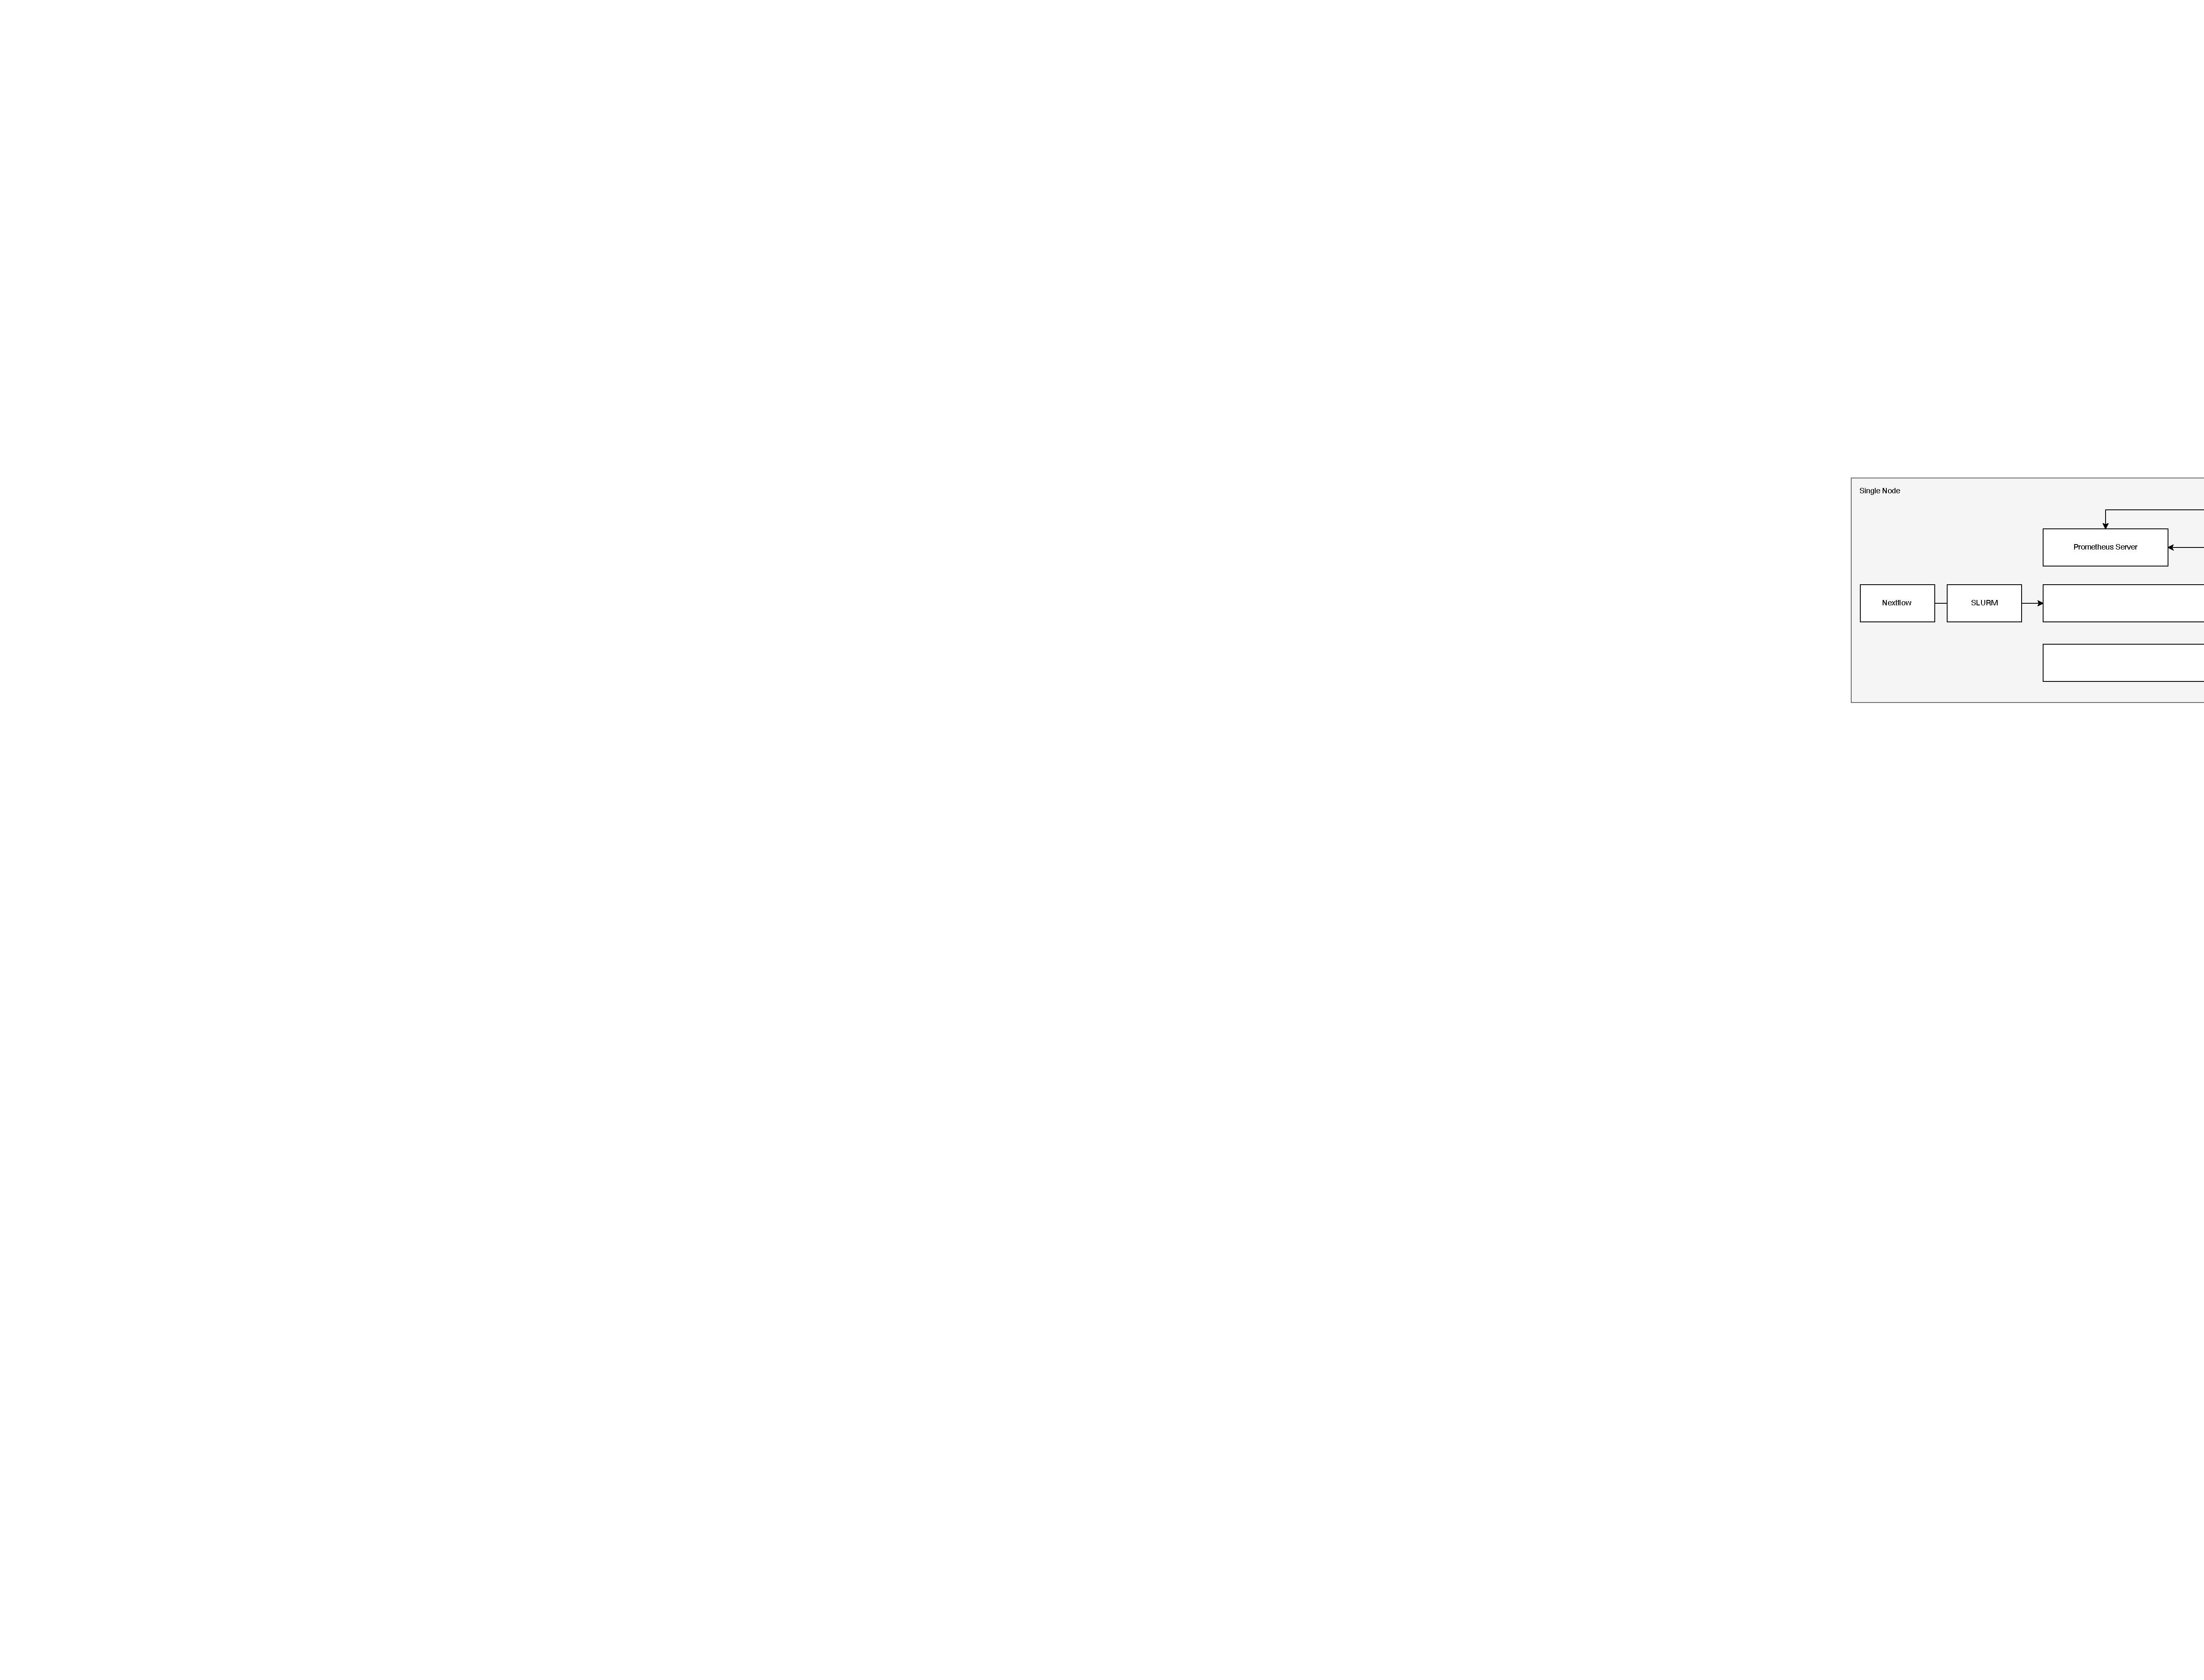
\includegraphics[scale=0.45]{fig/04/04-monitoring.pdf}
    \small
    \caption{Monitoring Client}
    \label{fig:04-monitoring}
    \tiny
    Schematic Overview of the Components of the Monitoring Client.
\end{figure}

Figure \ref{fig:04-monitoring} and Algorithm \ref{alg:monitoring} show the behavior of the monitoring client.

\begin{algorithm}[H]
    \caption{Event-Driven Monitoring and Metric Aggregation Framework}
    \label{alg:monitoring}
    \KwIn{Configuration $C$ defining monitoring targets}
    \KwOut{Aggregated container-level time-series metrics for each Nextflow process}

    \BlankLine
    initialize\_monitoring(C)\\
    init\_event\_listener()\\
    \While{true}{
        event $\gets$ wait\_for\_container\_event()\\
        meta $\gets$ extract\_metadata(event)\\
        \If{event.type = START}{
            register\_process(meta.id, meta.workflow\_label)
        }
        \If{event.type = TERMINATE}{
            metrics $\gets$ \{\}\\
            \ForEach{target $\in$ C.targets}{
                query $\gets$ build\_promql(target, meta.id, meta.time\_window)\\
                metrics[target] $\gets$ execute\_prometheus\_query(query)
            }
            data $\gets$ aggregate(metrics, meta.workflow\_label)\\
            store(data)
        }
    }
\end{algorithm}

% Algorithm Description
The algorithm outlined in Algorithm \ref{alg:monitoring} is designed to minimize monitoring overhead while ensuring that only relevant data is collected during workflow task execution. When a container start event is detected, the monitoring client extracts essential metadata—such as the container ID, the associated workflow label, and the start timestamp—and registers this information in an internal mapping to maintain a link between container identifiers and workflow tasks. When a termination event occurs, the client initiates a targeted data collection phase, querying only the relevant metrics for the specific container and execution period.

This event-driven approach ensures efficient monitoring by restricting data retrieval to the active lifecycle of workflow tasks. Furthermore, the monitoring client supports dynamic configuration of the metrics listed in Table \ref{tab:monitoring-metrics}, allowing users to define which metrics are collected and analyzed. This flexibility enables fine-grained, task-specific monitoring while maintaining low overhead and adaptability to different experimental requirements.

\subsection{Modelling the Co-location of Task Behavior based on Time-Series}
\label{sec:data_analysis}

This section corresponds to Steps 2, 3, and 4 in Figure \ref{fig:04-overview} and explains how the collected monitoring data is transformed into structured representations of task behavior. The focus lies on preparing and processing the raw time-series metrics to generate meaningful feature sets that can be used for two main purposes: identifying complementary tasks for co-location through clustering and building predictive models that capture the relationship between task behavior, runtime, and energy consumption.

\myparagraph{General Preprocessing of Raw Time-Series Data}
\label{sec:data_preprocessing_general}

The collected monitoring data is obtained as raw time-series files in CSV format and must therefore undergo several preprocessing steps before further analysis. The goal of this stage is to transform heterogeneous monitoring outputs into a consistent and structured representation that links system-level metrics to individual workflow tasks. The general preprocessing workflow includes the following steps:

% Paragraph about generic preprocessing of raw data
\begin{enumerate}
    \item Parsing of raw time-series CSV files.
    \item Alignment of timestamps across different sources.
    \item Merging of per-task data into unified records.
    \item Matching Entities between execution layer and workflow layer.
\end{enumerate}

% TODO: Add cursive for entities
% Explaining the pre-processing
During workflow execution, data is produced at multiple abstraction levels—from the resource manager down to container metrics. To transform this heterogeneous data into a unified, task-level format, a structured preprocessing pipeline was developed. First, all monitoring outputs are recursively traversed and scoped according to the desired data sources and metric types. The resulting directory tree is then filtered to retain only relevant metrics, such as task metadata and power measurements. Each dataset is subsequently split into per-task CSV files based on container identifiers.
As an anchor for this process, the started and died container tracking files are used, which record general container lifecycle information such as container names, identifiers, and timestamps. To establish a consistent mapping between workflow tasks and their corresponding container traces, entity matching is performed. Here, container lifecycle records—capturing task identifiers, container names, and working directories—serve as the linking mechanism between workflow-level entities and container-level monitoring data. The working directories are attached to every container trace, enabling a reliable cross-reference with workflow metadata extracted from SWMS trace files. This ensures that each monitored container is correctly associated with the corresponding workflow task, providing a coherent, task-centric dataset for subsequent analysis.

\subsubsection{Task Clustering for Contention-Aware Consolidation}
\label{sec:task_clustering}

Following the preprocessing and structuring of raw time-series data, we continue to address step 3 of the overall approach outlined in \ref{fig:04-overview}. This step focuses \textit{ShaReComp's} mechanics - task clustering as a means of identifying tasks that can be co-located without causing severe resource contention. The goal is to refine the processed monitoring data into representations that capture each task's characteristic resource usage patterns and to use these representations for forming complementary task groups. This clustering step forms the conceptual foundation for contention-aware consolidation.

\myparagraph{Preprocessing Raw Time-Series Data for Task-Clustering}
\label{sec:data_preprocessing_clustering}

To prepare the data for contention-aware task clustering, the processed time-series must be transformed into a compact yet expressive representation of each task's resource usage behavior. This ensures that the clustering algorithm can meaningfully capture similarities and differences between tasks across multiple resource domains. We therefore apply the following two main preprocessing steps prior to executing the clustering algorithm.

\begin{enumerate}
    \item \textbf{Peak-pattern construction}: For every task and monitored workload type, we first derive a peak time series: the raw per-second resource signal is resampled into three-second buckets and the maximum per bucket is retained. When two peak series must be compared, we truncate both to the shorter length so that correlation is computed on aligned vectors without padding artifacts.
    \item \textbf{Computing Workload-type affinity}: Different resource domains interfere to different degrees such as CPU vs CPU peaks are typically more contentious than CPU vs file I/O. We encode this by computing an affinity score between workload types which is described in \ref{sec:measuring_resource_contention}. High affinity means higher potential interference when peaks align; low affinity reflects benign coexistence.
\end{enumerate}

While the first step focuses on constructing consistent temporal representations of task behavior, the second step introduces a quantitative measure of how different workload types interact when co-located. To provide a clearer understanding of this relationship and its role in the clustering process, we examine the computation of workload-type affinity in more detail.

% Workload experiment design
\myparagraph{Measuring Resource Interference of Co-located Benchmarks}
\label{sec:measuring_resource_contention}

The measurement of resource contention follows a two-stage protocol that first establishes isolated baselines for each workload class and then repeats the same workloads under controlled co-location. In the baseline stage, CPU-bound, memory-bound, and file-I/O-bound benchmark containers are executed one at a time on pinned logical CPUs. Each run records a start and finish timestamp at microsecond resolution. In parallel, Deep-Mon is used to record the power time series for each container. After a run finishes, the power streams of the containers are retained, aligned to the container's lifetime, and summarized to a representative mean value.
After isolated benchmark execution we replay the same benchmarks in pairs to expose interference effects by CPU pinning. The experiment binds pairs of benchmarks to siblings on the same physical core to amplify shared-core effects. Each co-located container is measured in exactly the same way as in isolation, producing a matched set of durations and power summaries.

% Notation for the experiments.
In order to derive a workload affinity from the contention experiments we define contention effects to occur when co-located workloads exceed their duration and power consumption compared to their isolated measurements.
\[
    \textbf{Isolated and Co-located Metrics}
\]

For each workload \( i \in \{1,2\} \), let
\[
    t_i^{(iso)}, \; t_i^{(coloc)} \quad \text{denote the isolated and co-located runtimes,}
\]
\[
    P_i^{(iso)}, \; P_i^{(coloc)} \quad \text{denote the average isolated and co-located power consumption.}
\]

\[
    \textbf{Per-workload Slowdown Factors}
\]

The per-workload slowdowns are defined as
\[
    S_i^{(t)} = \frac{t_i^{(coloc)}}{t_i^{(iso)}},
    \qquad
    S_i^{(P)} = 1 + \log\!\left(
    \max\!\left( \frac{P_i^{(coloc)}}{P_i^{(iso)}}, 1 \right)
    \right),
\]
ensuring that both runtime and power slowdowns are
non-negative and at least one in value.

The mean slowdowns across the workload pair are
\[
    \bar{S}^{(t)} = \frac{S_1^{(t)} + S_2^{(t)}}{2},
    \qquad
    \bar{S}^{(P)} = \frac{S_1^{(P)} + S_2^{(P)}}{2}.
\]

A weighted average combines both effects:
\[
    \bar{S} =
    \alpha\, \bar{S}^{(t)} + (1 - \alpha)\, \bar{S}^{(P)},
    \quad \text{with } \alpha \in [0,1],
\]
where higher \(\alpha\) emphasizes runtime effects,
and lower \(\alpha\) gives more weight to power efficiency.

The final combined slowdown factor is
\[
    \bar{S}_{\text{final}} = \max(1, \bar{S}),
\]
guaranteeing that co-location never yields an apparent
speedup (values \(\ge 1\) indicate slowdown).

\[
    \textbf{Affinity Score}
\]

The affinity score \(A\) quantifies the degree of
interference between two co-located workloads.

First, compute pairwise affinity ratios:
\[
    A^{(t)} =
    \frac{t_1^{(coloc)} + t_2^{(coloc)}}
    {t_1^{(iso)} + t_2^{(iso)}},
    \qquad
    A^{(P)} =
    1 + \log\!\left(
    \max\!\left(
    \frac{P_1^{(coloc)} + P_2^{(coloc)}}
    {P_1^{(iso)} + P_2^{(iso)}},
    1
    \right)
    \right).
\]

A weighted average combines both effects:
\[
    A_{\text{raw}} =
    \alpha\, A^{(t)} + (1 - \alpha)\, A^{(P)},
    \qquad A_{\text{raw}} \ge 1.
\]

The normalized affinity score is then:
\[
    A =
    \frac{1 - \frac{1}{A_{\text{raw}}}}{\beta},
    \qquad A \in [0, 1],
\]
where \(\beta > 0\) controls scaling sensitivity.
Values of $A \approx 0$ indicate minimal interference,
while \(A \to 1\) signifies strong co-location interference.


\myparagraph{Algorithmic Approach to Task Consolidation}
\label{sec:algorithmic_approach_consolidation}

Building on the previously derived peak time-series representations and the computed workload-type affinity scores, we propose an algorithmic formulation of the consolidation, process.
Consolidation is formulated as a clustering problem with an important modification: rather than grouping tasks that are similar, the goal is to cluster tasks with complementary resource usage patterns to minimize contention during co-location. Building on the previously established notion of affinity that quantifies how strongly workloads interfere when sharing resources, the clustering process incorporates this measure directly into its distance metric. The distance between tasks increases when two tasks exert pressure on the same resources simultaneously, indicating potential contention, and decreases when their resource usage peaks complement one another.

Algorithm \ref{alg:task_distance_clustering} showcases the \textit{ShaReComp} task consolidation procedure developed in this work, integrating both the peak-pattern representations and affinity scores into a unified clustering process. The method first computes pairwise similarities between all task signatures, where each signature encodes the temporal evolution of multiple resource metrics. These similarities are weighted by the experimentally derived affinity values to reflect the degree of potential interference between workloads. The resulting similarity matrix thus provides a contention-aware view of task compatibility.
A percentile-based threshold is then applied to determine the stopping condition for cluster formation, ensuring that only task pairs with sufficiently low contention potential are merged. Finally, agglomerative clustering is executed using average linkage criterion to form consolidated task groups that exhibit complementary resource utilization.

% Algorithm for Task Consolidation in ShaReComp
\begin{algorithm}[H]
    \caption{ShaReComp - Task Consolidation Algorithm}
    \label{alg:task_distance_clustering}
    \SetKwFunction{Sim}{compute\_similarity}
    \SetKwFunction{Thresh}{percentile\_threshold}
    \SetKwFunction{Merge}{agglomerative\_merge}

    \KwIn{task signatures $\mathrm{sig}$, affinity weights $w$, percentile $\tau$, linkage}
    \KwOut{clusters $\mathcal{C}$}

    $S \gets$ \Sim($\mathrm{sig}$, $w$) \tcp*[r]{resource-aware similarity}
    $\theta \gets$ \Thresh($S$, $\tau$) \tcp*[r]{percentile-based stopping rule}
    $\mathcal{C} \gets$ \Merge($S$, $\theta$, linkage) \tcp*[r]{agglomerative clustering}

    \textbf{return } $\mathcal{C}$
\end{algorithm}

We examine each stage of Algorithm~\ref{alg:task_distance_clustering} in turn.

\textbf{Anti-similarity distance.} For any pair of tasks i,j, we iterate over their workload types and use two factors: (i) the affinity between the two types; (ii) the correlation between their corresponding peak series computed twice, once per type, to capture both sides of the pairing. We then aggregate these terms so that highly correlated peaks in high-affinity domains increase the distance, whereas low or negative correlations in low-affinity pairs decrease it. The result is a symmetric task distance matrix whose off-diagonal entries quantify how bad it would be to co-locate the two tasks, and whose diagonals are zero by definition.

% Notation for the distance formula
\[
    \textbf{Inter-Task Distance and Resource Correlation Model}
\]

To quantify the similarity and potential contention between two workloads
\( i \) and \( j \), we define a composite distance measure
that integrates both resource affinity and correlation of peak usage.
Each workload utilizes a set of resources
\( R = \{ \text{CPU}, \text{Memory}, \text{Disk}\} \),
yielding in total ten pairwise combinations of resource types across two tasks.
The distance term combines the precomputed affinity score with the
correlation of peak resource intensities.

\[
    D_{i,j}
    = \sum_{R_1, R_2}
    \Bigl(
    (\mathrm{aff\text{-}score}(R_1^i, R_2^j))
    \cdot
    \mathrm{Corr}(\mathrm{peak}\,R_1^i, \mathrm{peak}\,R_1^j)
    \cdot
    \mathrm{Corr}(\mathrm{peak}\,R_2^i, \mathrm{peak}\,R_2^j)
    \Bigr)
    \tag{1}
\]

where:
\begin{align}
    R_1^i, R_2^j & \; \text{denote resource types of workloads } i \text{ and } j,                           \\[4pt]
    \mathrm{Corr}(\mathrm{peak}\,R_1^i, \mathrm{peak}\,R_1^j)
                 & \; \text{is the Pearson correlation between the peak usages of resource } R_1
    \\[4pt]
    \mathrm{aff\text{-}score}(R_1^i, R_2^j)
                 & \in [0, 1] \text{ measures the degree of interference between } R_1^i \text{ and } R_2^j.
\end{align}

\[
    \textbf{Interpretation}
\]

The intuition behind this distance metric is to
\emph{promote dissimilar task pairings} for co-location.
If two workloads exhibit highly correlated peak usage on the same resources,
their corresponding correlation terms will be large,
thus increasing \( D_{i,j} \) and discouraging their co-location.
Conversely, tasks with uncorrelated or complementary resource peaks
yield smaller distance values and are therefore more suitable to merge.

The affinity score modulates this behavior:
smaller values of \( \mathrm{aff\text{-}score} \)
indicate lower interference between resource pairs,
which can offset strong peak correlations.

Finally, clustering proceeds by iteratively merging task clusters
whose inter-cluster distance satisfies:
\[
    D_{i,j} < \text{merge\_threshold}.
\]
This ensures that only compatible workloads, in terms of both
resource affinity and temporal peak correlation, are grouped together.

\textbf{Computing the merge threshold}. Because the distance matrix is data-dependent, we estimate a merge threshold directly from its empirical distribution. In our approach we select the 20th percentile on the raw distances as an automatic cut-level: any pair below this threshold is safe enough to consider for co-location, while pairs above it are kept apart.

\textbf{Agglomerative clustering with precomputed distances}. We run average-linkage agglomerative clustering on the precomputed distance matrix with the chosen distance threshold and no preset cluster count. This yields variable-sized clusters whose members are mutually non-contentious under our metric. Because we use a threshold rather than a fixed k, the method adapts to each workload mix, producing more or fewer groups as warranted by the observed interference structure.

\subsubsection{Predicting the Runtime and Energy Consumption of Task Clusters}
\label{sec:prediciton_kcca_rfr}

Following the reasoning of \cite{5644899}, we investigate whether the formed task clusters exhibit shared structures in terms of correlations between their time-series behavior and their corresponding energy and performance metrics. To this end, we adopt their proposed approach for preprocessing time-series data into temporal signatures on a per-task basis.

\myparagraph{Preprocessing Raw Time-Series Data for Predictive Modelling}
\label{sec:data_preprocessing_predictive}

Unlike the preprocessing described in Section \ref{sec:data_preprocessing_clustering}, the following procedure prepares the data specifically for step 4 of the overall approach shown in Figure \ref{fig:04-overview}, focusing on transforming raw time-series inputs into a form suitable for predictive modeling.

\begin{enumerate}
    \item Temporal signature construction.
          \subitem Sampling and smoothing.
          \subitem Equal-length normalization.
          \subitem Container-wise collation.
    \item Model Input Construction.
          \subitem Normalization and Scaling.
          \subitem Extraction of Input Features and Output Labels.
\end{enumerate}

% Formal notation

\[
    \textbf{Temporal Signature and Model Input Construction}
\]

We denote by \( \mathcal{T} = \{ T_1, T_2, \dots, T_N \} \) the set of
temporal signatures extracted from the monitored resource-usage profiles
of \( N \) workflow tasks.
Each task \( i \) is characterized by time-varying utilization traces
for the monitored resource dimensions
\[
    R = \{ \text{CPU}, \text{Memory}, \text{Disk} \}.
\]

\noindent
For each resource \( r \in R \) and task \( i \),
the temporal signature \( T_i^{(r)} \) is defined as a
coarse-grained summary of the normalized resource usage signal
\( x_i^{(r)}(t) \):
\[
    T_i^{(r)} =
    \bigl\langle
    p_{1,i}^{(r)},\;
    p_{2,i}^{(r)},\;
    \dots,\;
    p_{10,i}^{(r)}
    \bigr\rangle,
    \tag{1}
\]
where each component \( p_{k,i}^{(r)} \) represents the mean
usage value within segment \( k \) of the time-normalized
execution window (\( k = 1, \dots, 10 \)).
This yields a ten-dimensional vector describing the temporal pattern of
resource consumption.

\noindent
The feature vector for task \( i \) is obtained by concatenating
the resource-specific signatures:
\[
    x_i =
    \bigl[
    T_i^{(\text{CPU})},\;
    T_i^{(\text{Memory})},\;
    T_i^{(\text{Disk})},\;
    \bigr]
    \in \mathbb{R}^{d_x},
\]
where \( d_x = 3 \times 10 = 30 \) in this example configuration.

\[
    X =
    [x_1^\top, x_2^\top, \dots, x_N^\top]^\top
    \in \mathbb{R}^{N \times d_x}
\]
denotes the complete input matrix used for model training.

Similarly, for each task \( i \), the execution-level targets
(time and mean power consumption) are given by
\[
    y_i = [\,t_i,\, P_i\,] \in \mathbb{R}^2,
    \quad
    Y = [y_1^\top, y_2^\top, \dots, y_N^\top]^\top
    \in \mathbb{R}^{N \times 2}.
\]

\[
    \textbf{Example}
\]
Consider \( N = 3 \) workflow tasks with simplified
CPU and memory usage signatures
(each consisting of 3 representative pattern points for brevity):
\[
    \begin{array}{lcccccc}
        \toprule
        \text{Task}        &
        p_1^{(\text{CPU})} & p_2^{(\text{CPU})} & p_3^{(\text{CPU})} &
        p_1^{(\text{Mem})} & p_2^{(\text{Mem})} & p_3^{(\text{Mem})}                             \\
        \midrule
        1                  & 0.40               & 0.75               & 0.90 & 0.35 & 0.55 & 0.60 \\
        2                  & 0.20               & 0.50               & 0.70 & 0.25 & 0.40 & 0.50 \\
        3                  & 0.30               & 0.65               & 0.85 & 0.30 & 0.45 & 0.55 \\
        \bottomrule
    \end{array}
\]

Concatenating these signatures yields the input matrix
\[
    X =
    \begin{bmatrix}
        0.40 & 0.75 & 0.90 & 0.35 & 0.55 & 0.60 \\
        0.20 & 0.50 & 0.70 & 0.25 & 0.40 & 0.50 \\
        0.30 & 0.65 & 0.85 & 0.30 & 0.45 & 0.55
    \end{bmatrix},
    \quad
    Y =
    \begin{bmatrix}
        12.4 & 65 \\
        14.1 & 72 \\
        10.8 & 58
    \end{bmatrix}.
\]

Here, each row of \( X \) encodes the temporal resource-usage pattern
of a task, while \( Y \) provides the corresponding runtime and mean
power consumption used for model learning or correlation analysis.

This preprocessing yields: (i) a standardized and fixed-length feature matrix X that preserves per-metric usage distributions and (ii) a label matrix Y capturing runtime and energy

Building upon Algorithm \ref{alg:sharecomp} in Section \ref{sec:task_clustering}, we extend the \textit{ShaReComp} concept by linking task clustering with predictive modeling. This step introduces a follow-up procedure that uses the clustered task groups and their extracted temporal features from Section \ref{sec:prediciton_kcca_rfr} to model and predict the expected runtime and energy behavior of consolidated task clusters.

% Algorithm for prediction of task clusters.
\begin{algorithm}[H]
    \caption{ShaReComp — Prediction of Energy and Performance Behavior of Consolidated Task Clusters}
    \label{alg:sharecomp_prediction}
    \SetKwFunction{Aggregate}{sum\_cluster\_features}
    \SetKwFunction{Build}{build\_feature\_matrix}
    \SetKwFunction{Predict}{predict\_runtime\_and\_energy}

    \KwIn{task clusters $\mathcal{C}$, per-task signatures $\mathrm{sig}$, trained model $\mathcal{M}$ (KCCA or Random Forest)}
    \KwOut{predicted runtime energy pairs $\hat{Y} = \{ (\hat{t}_k, \hat{E}_k) \}$}

    \BlankLine
    \ForEach{cluster $C_k \in \mathcal{C}$}{
        $F_k \gets$ \Aggregate($\{\,\mathrm{sig}[t_i] \mid t_i \in C_k\,\}$) \tcp*[r]{sum task signatures to form cluster feature}
    }
    $X \gets$ \Build($\{F_k\}$) \tcp*[r]{construct consolidated feature matrix}

    \BlankLine
    \ForEach{cluster feature $X_k \in X$}{
        $(\hat{t}_k, \hat{E}_k) \gets$ \Predict($X_k$, $\mathcal{M}$)
    }
    \BlankLine
    \textbf{return } $\hat{Y} = \{ (\hat{t}_k, \hat{E}_k) \}_{k=1}^{|\mathcal{C}|}$
\end{algorithm}

The statistical models used in Algorithm \ref{alg:sharecomp_prediction} are described in the following.

\myparagraph{Kernel Canonical Correlation Analysis}
\label{sec:KCCA}

KCCA wants to identify relationships between task-specific features and their corresponding performance and energy characteristics. To achieve this, the dataset is divided into two parts: approximately 70\% of the tasks are used for training the models, while the remaining 30\% are reserved for testing and validation.

KCCA itself does not perform prediction but rather uncovers shared structures between task feature data performance outcomes. Through the data preprocessing described in the previous step, we prepare the feature matrices so that a regression model can generalize from the learned shared space to unseen inputs—for instance, the aggregated features of a new task cluster. We use KCCA to project both input and target data into a common latent space that captures nonlinear relationships between task resource usage and performance behavior.

% Notation
To capture nonlinear dependencies between the resource signatures
and performance power outcomes, we apply Gaussian kernels to both
input and output feature spaces.

KCCA seeks directions \(A\) and \(B\) in the
reproducing kernel spaces of \(K_x\) and \(K_y\)
that maximize the correlation between
\( K_x A \) and \( K_y B \).
This is expressed as the generalized eigenvalue problem:
\[
    \begin{bmatrix}
        0       & K_y K_x \\
        K_x K_y & 0
    \end{bmatrix}
    \begin{bmatrix}
        A \\ B
    \end{bmatrix}
    =
    \lambda
    \begin{bmatrix}
        K_x^2 & 0     \\
        0     & K_y^2
    \end{bmatrix}
    \begin{bmatrix}
        A \\ B
    \end{bmatrix}.
    \tag{2}
\]

Solving (2) yields paired canonical directions
\( (A, B) \) that define latent projections
\[
    X' = K_x A, \qquad Y' = K_y B,
\]
maximally correlated across the two feature spaces.
These projections represent a shared latent space
relating resource utilization dynamics to task performance and energy.

During training, we then fit a Kernel Ridge Regression model on the latent-space representations of the input features and the original, un-normalized target values Y (runtime and energy). This approach leverages KCCA's ability to transform unseen data into the same latent space, allowing KRR to predict concrete runtime and energy values for previously unseen X inputs. KRR is chosen because, as outlined in chapter \ref{sec:background_ml_lr}, it extends ordinary least squares regression by capturing nonlinear dependencies through kernel-based feature mappings.

\[
    \textbf{Illustrative Example}
\]
Consider three workflow tasks \( i = 1, 2, 3 \)
with aggregated temporal signatures over CPU and memory:
\[
    \begin{aligned}
        x_1 & = [0.40,\, 0.75,\, 0.90,\, 0.35,\, 0.55,\, 0.60], \\
        x_2 & = [0.20,\, 0.50,\, 0.70,\, 0.25,\, 0.40,\, 0.50], \\
        x_3 & = [0.30,\, 0.65,\, 0.85,\, 0.30,\, 0.45,\, 0.55].
    \end{aligned}
\]
Their corresponding runtime power outcomes are:
\[
    y_1 = [12.4,\, 65], \quad
    y_2 = [14.1,\, 72], \quad
    y_3 = [10.8,\, 58].
\]

KCCA maps both the temporal patterns \(x_i\)
and the performance power pairs \(y_i\)
into high-dimensional kernel spaces
and finds projections that maximize their mutual correlation.
In this example, the first canonical mode reveals that
tasks with higher sustained CPU activity
(\(x_1, x_3\))
correspond to lower execution time and reduced power consumption,
while the less efficient task (\(x_2\))
shows a distinct temporal signature characterized by
fluctuating utilization and higher runtime.

\myparagraph{Random Forest Regression}

To complement the KCCA model, we trained two non-parametric regressors based on Random Forests—one to predict mean task power and one to predict task runtime from the same preprocessed feature matrix. We reuse the exact same data as we did for the KCCA model as Random Forests perform well on both multivariate input and output data. The power model is trained on mean per-task energy-rate labels, while the runtime model uses task durations as targets. As a sanity check, we established simple baselines by predicting the training-set mean once for power and once for runtime on the test split. These baselines quantify the minimum improvement any learned model must exceed.

To illustrate this concept, we consider the following example.

% Example on how this looks
\myparagraph{Example on Predicting the Performance of Task Cluster with ShaReComp}
\label{sec:example_prediction_task_clusters}

Assume two clusters:
\[
    C_1 = \{t_1, t_2\}, \quad C_2 = \{t_3\},
\]
and each task has a CPU Memory signature with three pattern points:
\[
    t_1 = [0.4, 0.7, 0.9, 0.5, 0.6, 0.7], \quad
    t_2 = [0.3, 0.5, 0.8, 0.4, 0.5, 0.6], \quad
    t_3 = [0.2, 0.4, 0.6, 0.3, 0.4, 0.5].
\]
Applying \ref{alg:sharecomp_prediction} Cluster features are summed:
\[
    F_1 = t_1 + t_2 = [0.7, 1.2, 1.7, 0.9, 1.1, 1.3], \quad
    F_2 = t_3.
\]
Model predictions from both Kernel Ridge Regression or the Random Forest Regressor yield
\[
    \hat{Y} =
    \begin{bmatrix}
        10.8 & 62.5 \\
        14.2 & 75.1
    \end{bmatrix},
\]
representing predicted runtime (seconds) and energy (joules) per cluster.

\subsection{Simulation of Task Co-location during Workflow Execution}
\label{sec:simulation_environment}

We advance to steps 5 and 6 of the overall approach shown in Figure \ref{fig:04-overview}, where the previously developed concepts are embedded into a workflow execution environment. In this stage, the focus shifts from modeling and clustering individual tasks to simulating their co-location during execution, eventually allowing us to evaluate how these strategies affect overall performance and energy efficiency.

\myparagraph{Outline of Simulation Components}

\label{sec:design_pillars}
We build upon generic design pillars that structure the simulation environment.

% Figure with Simulator Design
\begin{figure}[H]
    \centering
    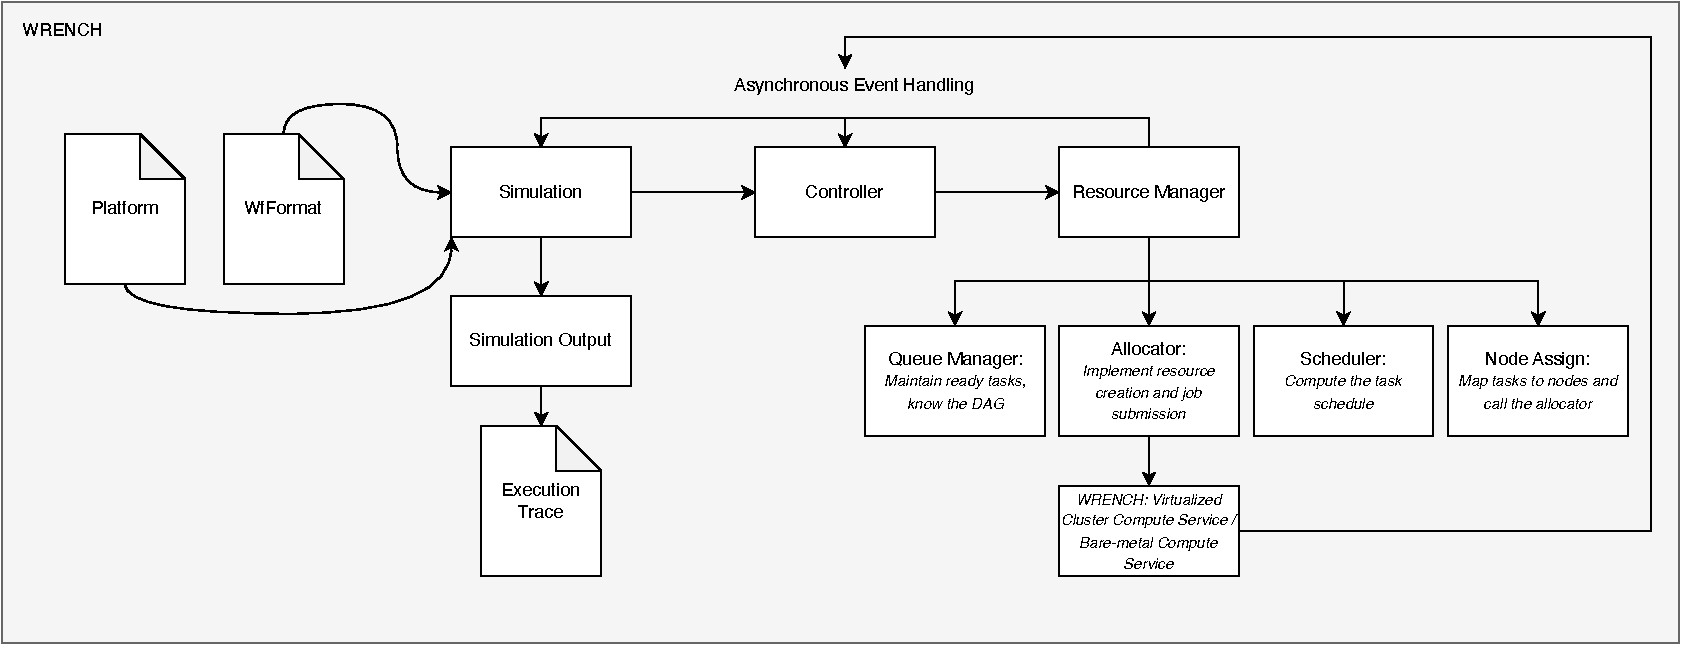
\includegraphics[scale=0.5]{fig/04/04-approach-sim.pdf}
    \small
    \caption{High-level Simulator-Design}
    \label{fig:04-sim-design}
    \tiny
    Simulator Design using WRENCH for studying Energy-aware Co-location of Scientific Workflow Tasks.
\end{figure}

The design of distributed HPC systems typically revolves around three fundamental mechanisms: resource allocation, queue management and dispatching, and job placement. As illustrated in Figure \ref{fig:04-sim-design}, these principles are adapted and integrated into our simulator through a dedicated controller component that interacts with a central resource manager. This resource manager orchestrates task scheduling, DAG-aware queue handling, task-to-node assignment, and the eventual allocation and execution of tasks on compute resources. Because the objective of this work is to analyze the effects of task co-location, the simulator's processing engine is designed with extensible interfaces that support alternative scheduling, mapping, and allocation strategies—from traditional First-In-First-Out (FIFO) execution to heuristic or energy-aware methods that emphasize beneficial co-location patterns.

\subsubsection{Embedding Task Co-location into Scheduling Heuristics}
\label{sec:heuristic_design}

Our algorithmic design for the resource manager, allocator, and scheduler components shown in Figure \ref{fig:04-sim-design} follows heuristic principles. Instead of formulating co-location within the scheduling process as an explicit optimization problem, we embed it through a set of simple, interpretable decision rules. We divide the task-to-node mapping process into two distinct stages, as illustrated in Figure \ref{fig:04-coloc-problem}. The simulation begins by launching the controller component, which invokes the resource manager. Through its queue management mechanism, the resource manager identifies all ready-to-run tasks that have no remaining dependencies. In the depicted example, tasks 1, 2, 4, 8, 11, 12, and 15 are selected for scheduling. For this process, we adopt list-scheduling algorithms, one of the most established heuristic approaches in workflow scheduling. These algorithms assign each task a priority or ranking based on topological and performance characteristics such as critical path length, estimated execution time, or communication cost. Tasks are then scheduled iteratively, with the highest-priority unscheduled task being mapped to an available resource until all ready tasks have been assigned.

% Figure with visualizing the co-loc problem
\begin{figure}[H]
    \centering
    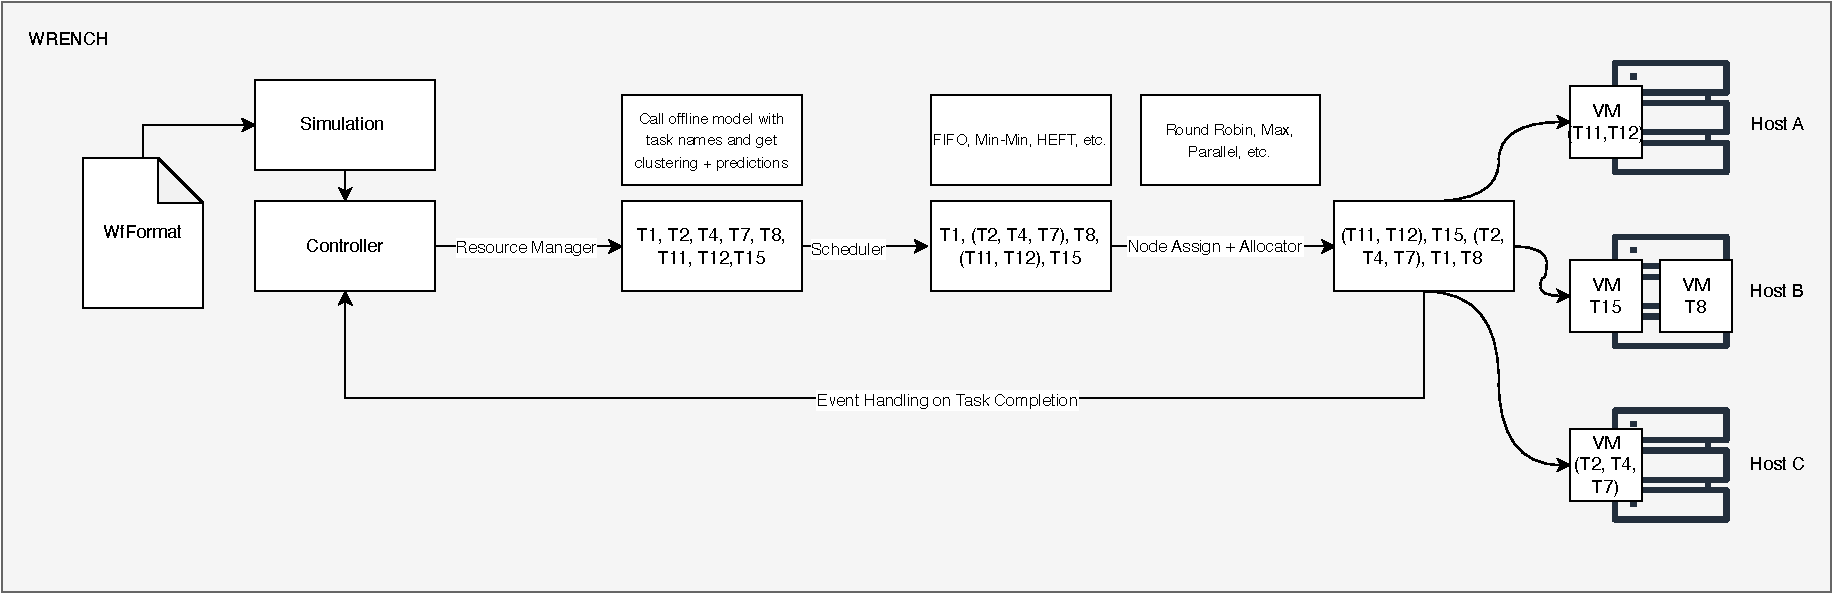
\includegraphics[scale=0.45]{fig/04/04-coloc-problem.pdf}
    \small
    \caption{Co-location embedded into Workflow Execution}
    \label{fig:04-coloc-problem}
    \tiny
    This figure shows a schematic example on how co-location is embedded in workflow execution.
\end{figure}

Since our goal is to map not individual tasks but clusters of tasks, we embed the retrieval of co-location information derived from \textit{ShaReComp} directly into this stage of the scheduling process. In the illustrated example, the co-location hints result in consolidated groups such as T1, (T2, T4, T7), T8, (T11, T12), and T15. After clustering, the next step is to determine which compute host can best accommodate each task group. To this end, we define an interface for node assignment strategies that can either prioritize hosts with the most idle compute cores or distribute task clusters evenly across all available nodes to ensure balanced utilization. Finally, the allocation component creates virtual machines for each task cluster and launches them on their designated hosts, completing the mapping and allocation workflow. Through this exemplified design, we establish a foundation that not only enables the embedding and study of the co-location problem within an execution environment but also allows for systematic comparison through modular component interfaces. The following section formally introduces the simulation environment and the system model that represents our algorithmic formulation of the co-location problem.

\newpage
% System Model that was used for the heuristic design.
\myparagraph{Simulation System Model}

\textbf{Workflow Properties}

Let the workflow be represented as a directed acyclic graph (DAG)
\[
    G = (T, E)
\]
where
\begin{itemize}
    \item $T = \{t_1, t_2, \dots, t_n\}$ denotes the set of \textbf{tasks}, and
    \item $E \subseteq T \times T$ denotes \textbf{data or control dependencies} between tasks.
\end{itemize}
A directed edge $(t_i, t_j) \in E$ indicates that task $t_j$ can start only after $t_i$ has completed.

\textbf{Task Properties}

Each task \( t_i \in T \) is associated with the following attributes:
\[
    \begin{array}{rcll}
        \text{req\_cores}(t_i) & \in & \mathbb{N}_{\ge 1} & \text{number of CPU cores required}, \\[4pt]
        \text{req\_mem}(t_i)   & \in & \mathbb{R}_{>0}    & \text{memory requirement in bytes.}
    \end{array}
\]

\textbf{Infrastructure Model}

Let \( \mathcal{H} = \{h_1, h_2, \dots, h_m\} \) denote the set of available \textbf{hosts},
where each host \( h_j \) is characterized by
\[
    C_j \in \mathbb{N}_{>0} \text{ (total number of cores)}, \qquad
    c(h_j) \in \mathbb{N}_{\ge 0} \text{ (current number of idle cores).}
\]

A \textbf{virtual machine (VM)} is represented as
\[
    v = (C_v, M_v, h_j),
\]
where \( C_v \) is the number of virtual cores, \( M_v \) the assigned memory,
and \( h_j \) the physical host on which it is instantiated.

The set of currently \textbf{ready tasks} (those whose dependencies are satisfied) is denoted by
\[
    \mathcal{Q} = \{t_1, t_2, \dots, t_k\}.
\]

\textbf{Resource Assignment}

A mapping of tasks to hosts and VMs is represented as
\[
    M = (h, \mathcal{T}_h, \text{colocMap}_h, \Phi_h),
\]
where
\begin{itemize}
    \item $h \in \mathcal{H}$ is the assigned host,
    \item $\mathcal{T}_h \subseteq T$ is the set of tasks mapped to $h$,
    \item $\text{colocMap}_h$ describes task clusters on $h$, and
    \item $\Phi_h$ represents associated file or data locations.
\end{itemize}
The set of mappings for an allocation interval is written as
\[
    \mathcal{M} = \{ M_1, M_2, \dots, M_p \}.
\]

\textbf{Task Co-location}

A \textbf{co-location mapping}, produced by a scheduler is defined as
\[
    \text{colocMap} = \{ (C_i, \mathcal{C}_i) \mid \mathcal{C}_i \subseteq T \},
\]
where $\mathcal{C}_i$ is a \textbf{cluster of tasks} to be executed together within a single virtual machine, ideally selected based on their resource affinity or complementary utilization patterns.

\textbf{Oversubscription}

An \textbf{oversubscription factor} $\alpha \in [0,1]$ allows up to
\[
    N_{\max}(h_j) = \lceil C_j (1 + \alpha) \rceil
\]
tasks to be scheduled concurrently on a VM on host $h_j$.


\textbf{Execution Dynamics}

At runtime:
\begin{itemize}
    \item \textbf{Node Assigners} determine host placement.
    \item \textbf{Schedulers} generate task queues and co-location groupings.
    \item \textbf{Allocators} instantiate and start VMs according to host-task mappings.
    \item The \textbf{Job Manager} executes tasks, monitors VM lifecycles, and updates resource states.
\end{itemize}

\newpage
We present the unified algorithm that governs the overall behavior of our simulation framework. This algorithm formalizes how workflow tasks are scheduled, assigned, and executed under different resource management strategies, including optional co-location support through \textit{ShaReComp}.

% Blueprint Algorithm 
\begin{algorithm}[H]
    \caption{ShaReComp Simulation - WRENCH Framework}
    \label{alg:sharecomp_unified}
    \KwIn{workflow \( G=(T,E) \), hosts \( \mathcal{H}=\{h_1,\dots,h_m\} \), scheduling policy \( \pi \), oversubscription factor \( \alpha \), optional co-location API \( \mathcal{S} \)}
    \KwOut{workflow executed with policy-driven scheduling, node assignment, and adaptive resource management}

    \BlankLine
    Initialize system state: host capacities, ready queue \( \mathcal{Q} \), and monitoring layer\\

    \While{workflow \( G \) not completed}{
        Update \( \mathcal{Q} \) with all newly ready tasks\\
        Perform \textbf{task scheduling}: prioritize tasks in \( \mathcal{Q} \) according to policy \( \pi \)\\
        Perform \textbf{node assignment}: select suitable host(s) \( h \in \mathcal{H} \) using \( \pi \)\\
        Perform \textbf{resource allocation}: determine allowed capacity \( n_{\max}=f(c(h),\alpha) \) and reserve resources\\
        \If{policy \( \pi \) supports co-location}{
            Optionally query \( \mathcal{S} \) to group tasks by affinity and launch them on shared VMs
        }\Else{
            Launch one task per VM on assigned host
        }
        Monitor execution and task completions\\
        Release resources and enqueue successors of completed tasks
    }
    \Return{workflow complete}
\end{algorithm}

To evaluate the effectiveness of the \textit{ShaReComp} approach, we define several scheduling and node assignment algorithms that differ in their treatment of resource sharing and task placement. All of these algorithms build upon the unified simulation blueprint presented in Algorithm \ref{alg:sharecomp_unified} and serve as comparative baselines. The first category of baselines executes each task in its own virtual machine, thereby avoiding any form of co-location. The second category enables task co-location by grouping multiple tasks within shared virtual machines and applying different host prioritization and allocation strategies. A third category extends this idea through controlled oversubscription, where more tasks are assigned to a virtual machine than the available reserved resources allow, deliberately inducing resource contention to test system robustness. Detailed algorithmic definitions are provided in the appendix, while \ref{cha:evaluation} discusses their comparative behavior in depth. The \textit{ShaRiff} algorithms build directly on top of these baselines, extending them with co-location awareness derived from \textit{ShaReComp}. In doing so, they replace random or static task grouping with data-driven consolidation decisions that account for resource affinity and contention characteristics.

\myparagraph{Algorithmic Examples of Task Mapping with guided Co-location}
\label{sec:co-location_strategies}

This section concludes our approach by introducing the integration of the \textit{ShaReComp} methodology into the workflow execution process. To this end, we design four scheduling algorithms collectively referred to as \textit{ShaRiff} (Share Resources if Feasible). Each \textit{ShaRiff} variant implements a distinct strategy for mapping consolidated task clusters onto available compute hosts, while the co-location decisions themselves are consistently guided by the \textit{ShaReComp} approach introduced in Section \ref{sec:task_clustering}. An overview of the four \textit{ShaRiff} variants and their respective strategies is provided in Table \ref{tab:shariff_overview}.

% Table with \textit{ShaRiff} Overview stuff.
\begin{table}[H]
    \centering
    \footnotesize
    \begin{tabularx}{\textwidth}{l p{10cm}}
        \toprule
        \textbf{Algorithm}      & \textbf{Type}                                                                                                  \\
        \midrule
        \textit{ShaRiff} 1      & Biggest Host first, parallel Host-backfilling and mapping of Task Clusters                                     \\
        \textit{ShaRiff} 2      & Biggest Host first, parallel Host-backfilling and mapping of Task Clusters with controlled VM Oversubscription \\
        \textit{ShaRiff} 3      & Round-Robin Assignment of Task Clusters, No parallelism                                                        \\
        \textit{ShaRiff} MinMin & Biggest Host first, parallel Host-backfilling and mapping of ordered Task Clusters                             \\
        \bottomrule
    \end{tabularx}
    \small
    \caption{Overview of the \textit{ShaRiff} scheduling variants that make use of ShaReComp.}
    \label{tab:shariff_overview}
\end{table}


In the following, we provide a detailed description of the behavior of each \textit{ShaRiff} algorithm, followed by its formal algorithmic representation.

% \textit{ShaRiff} 1
% Algorithm
\begin{algorithm}[H]
    \caption{ShaRiff 1 — Biggest Host first, parallel Host-backfilling and mapping of Task Clusters}
    \label{alg:sharecomp}
    \KwIn{workflow \( G=(T,E) \), hosts \( \mathcal{H}=\{h_1,\dots,h_m\} \), idle cores \( c(h_j) \), ShaReComp co-location API \( \mathcal{S} \)}
    \KwOut{all tasks \( t_i\in T \) executed with contention-aware co-location for improved efficiency and utilization}

    \BlankLine
    Initialize idle cores \( c(h_j)\gets C_j \) for all \( h_j\in\mathcal{H} \);
    Initialize ready queue \( \mathcal{Q} \) with all source tasks of \( G \) (FIFO order)

    \BlankLine
    \While{not all tasks \( t_i\in T \) completed}{
        \If{\( \mathcal{Q} \) is empty}{
            Wait until any task \( t_r \) completes;
            Release its cores: \( c(h(t_r)) \gets c(h(t_r)) + \text{req\_cores}(t_r) \);
            For each successor \( t_s \) of \( t_r \), enqueue \( t_s \) into \( \mathcal{Q} \) if all predecessors are completed;
            \textbf{continue}
        }

        Build available-host list \( L=\{\,h\in\mathcal{H}\mid c(h)>0\,\} \), sorted by \( c(h) \) descending;
        Initialize empty host task mapping list \( \mathcal{M} \);

        \BlankLine
        \ForEach{host \( h\in L \) and while \( \mathcal{Q} \) not empty}{
            Select up to \( c(h) \) ready tasks from \( \mathcal{Q} \) into \( \mathcal{T}_h \);
            Compute file-location map \( \Phi(\mathcal{T}_h) \);
            Query ShaReComp API: \( \text{colocMap} \gets \mathcal{S}(\mathcal{T}_h) \) \tcp*[r]{returns co-location groups}
            Add mapping \( (h,\mathcal{T}_h,\Phi(\mathcal{T}_h),\text{colocMap}) \) to \( \mathcal{M} \);
        }

        \BlankLine
        \ForEach{mapping \( (h,\mathcal{T}_h,\Phi,\text{colocMap}) \in \mathcal{M} \)}{
            \ForEach{group \( \mathcal{C}_k \in \text{colocMap} \)}{
                \( C_{\text{req}} \gets \text{sum(req\_cores}(\mathcal{C}_k)) \);
                \( M_{\text{req}} \gets \text{sum(req\_mem}(\mathcal{C}_k)) \);
                Allocate \( v_h = (C_{\text{req}}, M_{\text{req}}, h) \);
                Launch all \( t \in \mathcal{C}_k \) on \( v_h \);
                \( c(h) \gets \max(0, c(h) - C_{\text{req}}) \);
                Remove \( \mathcal{C}_k \) from \( \mathcal{Q} \);
            }
        }

        \BlankLine
        Wait until any task \( t_r \) completes;
        Release its cores: \( c(h(t_r)) \gets c(h(t_r)) + \text{req\_cores}(t_r) \);
        \If{no active tasks remain on its VM}{ Destroy VM }
        For each successor \( t_s \) of \( t_r \): if all predecessors are completed, enqueue \( t_s \) into \( \mathcal{Q} \);
    }
    \Return{workflow complete}

\end{algorithm}

This variant implements \textit{ShaRiff} 1, which augments a FIFO pipeline with the external co-location adviser \textit{ShaReComp} and a cluster-aware allocator. Tasks are dequeued in strict arrival order. Before placement, the scheduler invokes \textit{ShaReComp} with the current set of ready tasks and receives clusters of jobs that are computed to co-locate well. The node-assignment stage then ranks hosts by descending idle-core capacity and fills the largest host first. It forms a batch of up to that hosts idle cores and attaches the \textit{ShaRiff} cluster map to the batch. If tasks remain, it proceeds to the next host in the ranked list. A small queue path ensures dispatch even when only a few tasks are available.
The allocator realizes the advisers plan one VM per recommended cluster on the chosen host. For each multi-task cluster, it provisions a VM whose vCPU count and memory equal the sum of the clustered tasks declared requirements, starts the VM, and submits the tasks to that same virtual compute service. Singleton clusters are grouped into a shared VM on the host to avoid VM fragmentation.
Conceptually, \textit{ShaRiff} preserves FIFO ordering and capacity-ranked host filling, but replaces random batching with adviser-driven clustering.

% \textit{ShaRiff} 2
% Algorithm
\begin{algorithm}[H]
    \caption{ShaRiff 2 — Biggest Host first, parallel Host-backfilling and mapping of Task Clusters with controlled VM Oversubscription}
    \label{alg:sharecomp_oversub}
    \KwIn{workflow \( G=(T,E) \), hosts \( \mathcal{H}=\{h_1,\dots,h_m\} \), idle cores \( c(h_j) \), oversubscription factor \( \alpha \), ShaReComp co-location API \( \mathcal{S} \)}
    \KwOut{workflow executed with affinity-based co-location, maximal host parallelism, and safe oversubscription}

    \BlankLine
    Initialize idle cores \( c(h_j)\gets C_j \) for all \( h_j\in\mathcal{H} \)
    Initialize ready queue \( \mathcal{Q} \) with all source tasks of \( G \) (FIFO order)

    \BlankLine
    \While{not all tasks \( t_i\in T \) completed}{
        \If{\( \mathcal{Q} \) is empty}{
            Wait until any task \( t_r \) completes
            Release its cores: \( c(h(t_r)) \gets c(h(t_r)) + \text{req\_cores}(t_r) \)
            For each successor \( t_s \) of \( t_r \), enqueue \( t_s \) into \( \mathcal{Q} \) if all predecessors are completed\\
            \textbf{continue}
        }

        Build available-host list \( L=\{\,h\in\mathcal{H}\mid c(h)>0\,\} \), sorted by \( c(h) \) descending
        Initialize empty host task mapping list \( \mathcal{M} \)

        \BlankLine
        \ForEach{host \( h\in L \) and while \( \mathcal{Q} \) not empty}{
            Compute oversubscription limit \( n_{\max} = \lceil c(h) \times (1 + \alpha) \rceil \)
            Select up to \( n_{\max} \) ready tasks from \( \mathcal{Q} \) into \( \mathcal{T}_h \)
            Compute file-location map \( \Phi(\mathcal{T}_h) \)
            Query ShaReComp API: \( \text{colocMap} \gets \mathcal{S}(\mathcal{T}_h) \) \tcp*[r]{returns co-location groups}
            Add mapping \( (h,\mathcal{T}_h,\Phi(\mathcal{T}_h),\text{colocMap}) \) to \( \mathcal{M} \)
        }

        \BlankLine
        \ForEach{mapping \( (h,\mathcal{T}_h,\Phi,\text{colocMap}) \in \mathcal{M} \)}{
            \ForEach{group \( \mathcal{C}_k \in \text{colocMap} \)}{
                \( C_{\text{req}} \gets \text{sum(req\_cores}(\mathcal{C}_k)) \)
                \( M_{\text{req}} \gets \text{sum(req\_mem}(\mathcal{C}_k)) \)
                \If{\( C_{\text{req}} > c(h) \)}{
                    Allocate \( v_h = (c(h), M_{\text{req}}, h) \); \tcp*[r]{oversubscription active}
                }
                \Else{
                    Allocate \( v_h = (C_{\text{req}}, M_{\text{req}}, h) \)
                }
                Launch all \( t \in \mathcal{C}_k \) on \( v_h \)
                \( c(h) \gets \max(0, c(h) - C_{\text{req}}) \)
                Remove \( \mathcal{C}_k \) from \( \mathcal{Q} \)
            }
        }

        \BlankLine
        Wait until any task \( t_r \) completes
        Release its cores: \( c(h(t_r)) \gets c(h(t_r)) + \text{req\_cores}(t_r) \)
        \If{no active tasks remain on its VM}{ Destroy VM }
        For each successor \( t_s \) of \( t_r \): if all predecessors are completed, enqueue \( t_s \) into \( \mathcal{Q} \)
    }
    \Return{workflow complete}
\end{algorithm}

% \textit{ShaRiff} 2
This variant extends \textit{ShaRiff} 1 by controlled oversubscription during placement and VM sizing. Tasks are dequeued in arrival order. Before dispatch, the scheduler queries ShaReComp with the current ready set and receives clusters of tasks pcomputed to co-locate well. Hosts are ranked by descending idle-core capacity; the assigner then fills the largest host first with a batch whose size may exceed the hosts free cores by a fixed factor of in our example 25\%. If tasks remain, it proceeds to the next host and repeats.
The allocator implements the advisers plan one VM per cluster on the chosen host, but with oversubscription semantics. For multi-task clusters, it provisions a VM whose vCPU and memory equal the sum of the clusters requests—even if that exceeds the hosts currently free cores. For single task clusters collected on the same host, it provisions a shared VM and caps vCPUs at the hosts free cores when necessary.
Because ShaReComp groups complementary tasks, oversubscription holds the potential to translate into higher throughput and energy efficiency. However, when clustered tasks are less complementary, contention can surface, making this variant an explicit trade-off between utilization and interference.

% \textit{ShaRiff} 3
% Algorithm

\begin{algorithm}[H]
    \caption{ShaRiff 3 — Round-Robin Assignment of Task Clusters, No parallelism}
    \label{alg:sharecomp_rr}
    \KwIn{workflow \( G=(T,E) \), hosts \( \mathcal{H}=\{h_1,\dots,h_m\} \), idle cores \( c(h_j) \), ShaReComp co-location API \( \mathcal{S} \)}
    \KwOut{tasks executed using round-robin host selection with affinity-based VM co-location}

    \BlankLine
    Initialize idle cores \( c(h_j)\gets C_j \) for all \( h_j\in\mathcal{H} \)
    Initialize ready queue \( \mathcal{Q} \) with all source tasks of \( G \) (FIFO order)
    Initialize round-robin index \( r \gets 0 \)

    \BlankLine
    \While{not all tasks \( t_i\in T \) completed}{
        \If{\( \mathcal{Q} \) is empty}{
            Wait until any task \( t_r \) completes
            Release its cores: \( c(h(t_r)) \gets c(h(t_r)) + \text{req\_cores}(t_r) \)
            For each successor \( t_s \) of \( t_r \), enqueue \( t_s \) into \( \mathcal{Q} \) if all predecessors are completed\\
            \textbf{continue}
        }

        Select next host \( h = \mathcal{H}[r \bmod |\mathcal{H}|] \)
        Update round-robin index: \( r \gets (r + 1) \bmod |\mathcal{H}| \)
        Retrieve available cores \( C = c(h) \)
        Select up to \( C \) ready tasks from \( \mathcal{Q} \) into \( \mathcal{T}_h \)
        Query ShaReComp API: \( \text{colocMap} \gets \mathcal{S}(\mathcal{T}_h) \) \tcp*[r]{returns co-location groups}

        \BlankLine
        \ForEach{group \( \mathcal{C}_k \in \text{colocMap} \)}{
            \( C_{\text{req}} \gets \text{sum(req\_cores}(\mathcal{C}_k)) \)
            \( M_{\text{req}} \gets \text{sum(req\_mem}(\mathcal{C}_k)) \)
            Allocate \( v_h = (C_{\text{req}}, M_{\text{req}}, h) \)
            Launch all \( t \in \mathcal{C}_k \) on \( v_h \)
            \( c(h) \gets \max(0, c(h) - C_{\text{req}}) \)
            Remove \( \mathcal{C}_k \) from \( \mathcal{Q} \)
        }

        \BlankLine
        Wait until any task \( t_r \) completes
        Release its cores: \( c(h(t_r)) \gets c(h(t_r)) + \text{req\_cores}(t_r) \)
        \If{no active tasks remain on its VM}{ Destroy VM }
        For each successor \( t_s \) of \( t_r \): if all predecessors are completed, enqueue \( t_s \) into \( \mathcal{Q} \)
    }
    \Return{workflow complete}
\end{algorithm}

\textit{ShaRiff} 3 combines round-robin first-fit placement with \textit{ShaReComp}-guided intra-VM co-location. The scheduler releases tasks strictly in arrival order. The node-assignment component scans hosts in round-robin fashion and picks the first host reporting at least one idle core. It then pulls up to that hosts idle-core capacity worth of ready tasks and queries \textit{ShaReComp} for a co-location plan over this batch.
The allocator realizes \textit{ShaReComp's} plan one VM per suggested cluster on the chosen host. For each multi-task cluster, it sizes the VM by summing vCPU and memory requirements of the clusters tasks, starts the VM, and submits all cluster tasks to the same virtual compute service.
Conceptually, the policy is first-fit host, adviser-driven packing. Unlike the other variants, this strategy does not oversubscribe cores. It fills only the currently free capacity of the first eligible host and relies on \textit{ShaReComp's} clustering to raise utilization and efficiency through informed co-location.


% MinMin extension
This scheduler variant extends the \textit{ShaRiff} framework with a MinMin ordering layer, a classical heuristic from list scheduling. Instead of operating on individual tasks, it applies the MinMin principle to task clusters generated by \textit{ShaReComp's} co-location analysis. At each scheduling interval, the scheduler requests a new clustering of ready tasks, queries the prediction service using the models introduced in \ref{sec:prediciton_kcca_rfr} with \ref{alg:sharecomp_prediction} for estimated runtimes, and orders clusters in ascending order of predicted execution time. The \textit{ShaRiff} node assignment and VM allocator then manage placement and resource provisioning. In essence, this forms a MinMin scheduler over co-located clusters, combining \textit{ShaRiff's} affinity-based co-location with prediction-guided execution ordering to minimize queueing delays and improve overall workflow completion time.

\newpage
% ShaRiff 1 - MinMin
\begin{algorithm}[H]
    \caption{ShaRiff 1 MinMin — Biggest Host first, parallel Host-backfilling and ordered mapping of Task Clusters}
    \label{alg:shariff_minmin}
    \KwIn{workflow \( G=(T,E) \), hosts \( \mathcal{H}=\{h_1,\dots,h_m\} \), idle cores \( c(h_j) \), ShaReComp co-location API \( \mathcal{S} \), prediction service \( \mathcal{P} \)}
    \KwOut{all tasks \( t_i\in T \) executed with predictive ordering and contention-aware co-location}

    \BlankLine
    Initialize idle cores \( c(h_j)\gets C_j \) for all \( h_j\in\mathcal{H} \)
    Initialize ready queue \( \mathcal{Q} \) with all source tasks of \( G \) (FIFO order)

    \BlankLine
    \While{not all tasks \( t_i\in T \) completed}{
        \If{\( \mathcal{Q} \) is empty}{
            Wait until any task \( t_r \) completes\\
            Release its cores: \( c(h(t_r)) \gets c(h(t_r)) + \text{req\_cores}(t_r) \)
            For each successor \( t_s \) of \( t_r \), enqueue \( t_s \) into \( \mathcal{Q} \) if all predecessors are completed\\
            \textbf{continue}
        }

        Build available-host list \( L=\{\,h\in\mathcal{H}\mid c(h)>0\,\} \), sorted by \( c(h) \) descending
        Initialize empty host-task mapping list \( \mathcal{M} \)

        \BlankLine
        \ForEach{host \( h\in L \) and while \( \mathcal{Q} \) not empty}{
            Select up to \( c(h) \) ready tasks from \( \mathcal{Q} \) into \( \mathcal{T}_h \)
            Compute file-location map \( \Phi(\mathcal{T}_h) \)\\
            Query ShaReComp API: \( \text{colocMap} \gets \mathcal{S}(\mathcal{T}_h) \) \tcp*[r]{returns co-location groups}
            Add mapping \( (h,\mathcal{T}_h,\Phi(\mathcal{T}_h),\text{colocMap}) \) to \( \mathcal{M} \)
        }

        \BlankLine
        \tcp{Predictive MinMin ordering based on estimated runtimes}
        Query prediction API: \( \text{predictions} \gets \mathcal{P}(\mathcal{M}) \)
        Sort mappings \( \mathcal{M} \) by ascending predicted runtime: \( \mathcal{M}_{sorted} = \text{sort}_{asc}(\mathcal{M}, \text{key}=r_i) \)

        \BlankLine
        \ForEach{mapping \( (h,\mathcal{T}_h,\Phi,\text{colocMap}) \in \mathcal{M}_{sorted} \)}{
            \ForEach{group \( \mathcal{C}_k \in \text{colocMap} \)}{
                \( C_{\text{req}} \gets \text{sum(req\_cores}(\mathcal{C}_k)) \)
                \( M_{\text{req}} \gets \text{sum(req\_mem}(\mathcal{C}_k)) \)
                Allocate \( v_h = (C_{\text{req}}, M_{\text{req}}, h) \)
                Launch all \( t \in \mathcal{C}_k \) on \( v_h \)
                \( c(h) \gets \max(0, c(h) - C_{\text{req}}) \)
                Remove \( \mathcal{C}_k \) from \( \mathcal{Q} \)
            }
        }

        \BlankLine
        Wait until any task \( t_r \) completes\\
        Release its cores: \( c(h(t_r)) \gets c(h(t_r)) + \text{req\_cores}(t_r) \)
        \If{no active tasks remain on its VM}{ Destroy VM }
        For each successor \( t_s \) of \( t_r \): if all predecessors are completed, enqueue \( t_s \) into \( \mathcal{Q} \)
    }
    \Return{workflow complete}
\end{algorithm}